
\chapter{语音识别中的解码搜索问题}
\label{chap:intro2}

本章中,我们首先介绍基本的维特比解码搜索算法,而后引入其在语音识别中的应用。我们对语音识别中的解码搜索问题及其当前解决方案进行了详细介绍。这些不同的技术流派包括同步和非同步之分,以及动态和静态之分。我们对近十年主流的加权有限状态机技术进行了重点介绍。基于上面的介绍,我们总结了当前解码器研究中的待解决问题,以及上一章中深度序列学习模型所带来的研究机遇。后续本论文的一系列工作将基于本章针对解码器的分析,讨论和总结。


\section{维特比解码搜索算法}
\label{chap:intro2-viterbi}

维特比算法是一种动态规划算法,用于寻找维特比路径,其对应于最有可能产生观测事件的序列,即隐含状态序列。这一算法最早由安德鲁·维特比(Andrew Viterbi)在1967年提出,用于在数字通信链路中解卷积以消除噪音。 此算法被广泛应用于GSM和CDMA数字蜂窝网络、拨号调制解调器、深空通信、卫星和802.11无线网络中的解卷积码。另一大类应用为计算语言学和生物信息学,以及语音识别和关键字检测。例如在语音识别中,声音信号作为观察到的事件序列,而文本字符串,被看作是隐含的产生声音信号的给定原因,因此可对声音信号应用维特比解码搜索算法寻找最有可能的文本字符串序列。

假设给定隐式马尔可夫模型(HMM)状态空间 S, 初始处于状态i 的概率 $\pi_{i}$ 以及转移概率 $a_{i,j}$,其对应于从状态i转移到状态j的概率。同时我们观测到输出序列 $\mathbf{o}_{1},\dots ,\mathbf{o}_{T}$。 其对应的产生该观察序列的相应隐状态 $s_{1},\dots ,s_{T}$ 可以由递推关系得到。

\begin{equation}
\begin{split}
V_{1,j}= {P} {\big (}\mathbf{o}_{1}\ |\ j{\big )}\cdot \pi _{j}
\end{split}
\end{equation}
\begin{equation}
\begin{split}
V_{t,j}=\max _{i\in S}\left( {P} {\big (}\mathbf{o}_{t}\ |\ j{\big )}\cdot a_{i,j}\cdot V_{t-1,i}\right)
\end{split}
\end{equation}

这里的$ {P} {\big (}\mathbf{o}_{t}\ |\ j{\big )}$ 表示状态j的输出概率,$V_{t,j}$表示前 t 步最终状态为 j 的观测结果最有可能对应的状态序列的概率。通过保存向后指针记住在第二个等式中用到的状态 i 可以获得维特比路径。声明一个函数$\mathrm {Ptr} (x_{t},t)$ ,它返回若 $t>1$ 时计算 $V_{t,j}$ 用到的上一个隐状态i,这样:

\begin{equation}
\begin{split}
s_{T}=\arg \max _{i\in S}(V_{T,i})
\end{split}
\end{equation}
\begin{equation}
\begin{split}
s_{t-1}=\mathrm {Ptr} (s_{t},t)
\end{split}
\end{equation}

该算法复杂度为 $O(T\times \left|{S}\right|^{2})$。一个更好的估计存在于迭代只针对那些可以连接到当前状态的下一个状态当中,那么算法复杂度为,

\begin{equation}
\begin{split}
\label{equ:viterbi-cmp}
O(T\times (\left|{S}\right|+\left|{E}\right|))
\end{split}
\end{equation}
 其中的E 表示图中所存在的边,S表示图中所有的状态。

\section{语音识别中的解码搜索问题}
\label{sec:decode}

语音信号的识别既是一个模式识别问题,也包含相应的推理搜索问题。前一个问题对各种语音信号的、语言现象进行数学表示和描述,在基于统计学习的模式识别框架下进行建模,这决定了语音信号的识别系统可达到识别准确度的上限。而后一个问题在给定模型情况底下,研究如何高效地将输入语音信号的和模型相匹配,推理搜索得到最优识别结果,这决定了识别速度和实际可达的识别准确度。
在语音信号的识别的推理搜索阶段,解码器功能是对声学模型计算出的声学特征概率和语言模型计算出的语言概率进行组合来得到最大概率的词序列。

在语音识别中,声音信号作为观察到的事件序列,而文本字符串,被看作是隐含的产生声音信号的给定原因,因此可对声音信号应用维特比解码搜索算法寻找最有可能的文本字符串序列,称为语音识别的推理搜索阶段。
如公式\ref{eq:asr}所示,解码的过程是在给定声学模型和语言模型之后寻找拥有最大概率路径。

\begin{eqnarray}
\mathbf{w}^* &=& \arg \max_{\mathbf{w} \in \mathcal{H}}p(\mathbf{O}|\mathbf{w})P(\mathbf{w}) \\
&=& \arg \max_{\mathbf{w} \in \mathcal{H}} \sum_{\mathbf{s}} P(\mathbf{s}|\mathbf{w})p(\mathbf{O}|\mathbf{s})P(\mathbf{w})
\end{eqnarray}
这里$\mathbf{s}$是所有可能的状态序列,$P(\mathbf{w})$通过语言模型计算,$P(\mathbf{s}|\mathbf{w})p(\mathbf{O}|\mathbf{s})$通过声学模型计算。正如我们在章节\ref{sec:calc_like}中讨论过的,这一似然可以通过前向后向算法进行计算。然而,因为候选词序列可能性过于庞大,无法通过对每个候选进行前向后向算法来计算似然。因此,实际中通常利用最大概率的状态路径来近似整个概率,即:
\begin{equation}
\label{eq:decode}
\mathbf{w}^* = \arg \max_{\mathbf{w} \in \mathcal{H}} \max_{\mathbf{s}} P(\mathbf{s}|\mathbf{w})p(\mathbf{O}|\mathbf{s})P(\mathbf{w})
\end{equation}
这样我们可以通过利用动态规划(Dynamic Programming, DP)的方法计算出拥有最大概率状态序列,然后以此推理搜索出词序列,这一算法被称为Viterbi算法~\cite{viterbi1967error}。另$\phi_i(t)$表示在时刻$t$且输出了部分从$\mathbf{o}_1$至$\mathbf{o}_t$声学特征后停留在状态$i$的最大概率。它可以利用递归来计算:
\begin{equation}
    \phi_i(t)=\max_j\{\phi_j(t-1)a_{j,i}\}b_i(\mathbf{o}_t)
\end{equation}
这里$a_{i,j}$是状态转移概率,$b_i(\mathbf{o}_t)$是状态输出概率。最终:
\begin{equation}
    p(\mathbf{O}|\mathbf{w}) \approx \phi_{N}(T+1) = \max_i\{\phi_i(T)a_{i,N}\}
\end{equation}
Viterbi算法可以很容易扩展到连续语音信号的识别,一种扩展后的Viterbi算法也被称为令牌传递(Token Passing)算法~\cite{young2002htk}。在这一算法中,每一个状态将不仅仅保留一个最优路径,而是保存一部分个令牌。每一个令牌记录着某个候选词序列在第$t$时刻到达状态$i$的最优路径。在到达一个词边界时,语言模型的分数会直接加上。在整个观测序列结束时,拥有最大概率的令牌将被提取出来回溯其整个HMM序列。

即使利用了令牌传递算法,在大词汇连续语音信号的识别中,传播所有令牌搜索代价依然十分庞大。为了减少计算代价,通常会利用基于集束搜索(beam search)剪枝方法。在这一方法中,所有$\phi_i(t)$低于$i$中最大概率减去一个阈值的令牌都会被移除,这一阈值也被称为集束(beam)宽度,剪枝也可以在加完语言模型之后进行。虽然beam搜索方法可以显著减少计算量,但是有可能在早期阶段利用了过窄的beam宽度而剪去了真正最优路径导致识别错误。所以,beam宽度设置需要在减少计算量和提升识别准确率之间进行均衡。

语言分数和声学分数之间动态范围的区别也是需要考虑问题,通常会分别对声学分数和语言分数进行缩放。另外需对插入错误添加额外惩罚,从而均衡词错误率中的插入和删除错误比例,因而最终语音信号的识别中利用的准则是:
\begin{equation}
\mathbf{w}^* = \arg \max_{\mathbf{w} \in \mathcal{H}} \{\log p(\mathbf{O}|\mathbf{w}) + \alpha \log P(\mathbf{w}) + \beta L_{\mathbf{w}}\}
\end{equation}
这里$\alpha$是语言模型分数缩放系数,$\beta$是插入错误惩罚系数,$L_{\mathbf{w}}$是词序列长度。
通常会选择最大概率路径作为识别结果,也可以输出一部分候选结果然后用更强的语言模型来重新评价(比如利用神经网络语言模型)。这一候选的路径一般利用N-best列表~\cite{schwartz1990n}或者利用能包含更多信息的词级词图(Word Graph/Word Lattice)~\cite{ortmanns1997word}。

在语音信号的识别推理搜索阶段,解码器是语音信号的识别系统的核心和灵魂,所有信息都汇集于此。它将不同来源、 不同层次、 不同性质的知识和信息关联在一起,使它们互相之间取长补短, 从而得到正确的语音信号的识别结果。因此,如何将各种性质不同的信息有机融合是解码网络和解码算法设计中必须认真研究和解决的重要问题之一。
从解码器的作用来看,它不仅是验证语音信号识别中各种理论,模型和算法正确性的基本实验平台,也是构建实际系统的基础。因此,在解码器设计中,还必须考虑到研究的便利性和工程的实际应用。
近些年来,基于加权有限状态机(Weighted Finite-State Transducer, WFST)~\cite{mohri2002weighted}的搜索解码器被愈加多的人采用,它的优点是可以将语言模型提前地融合成一个统一搜索网络,从而在解码时加快解码速度。

语音识别系统可以分为关键词检测,孤立词识别,语法网络识别,大词汇连续语音识别和基于神经网络语音模型的大词汇连续语音识别,下面我们将对它们中的解码搜索问题进行逐一介绍。

\subsection{关键词检测}
\label{chap:intro-kws-dec}

%综述关键词检测
关键词检测(KWS)是语言识别最主要的应用之一,它的目标是得到一个高准确度和高效率的识别器,用于检测特定的一些关键词在语音中的出现。
KWS可以被用于声学数据挖掘~\cite{zhou2005data}, 低资源的音频检索~\cite{shen2009comparison}, 
语料库检索~\cite{garofolo2000trec} 和 唤醒词识别~\cite{chen2014small}。

\subsubsection{关键词检测模型的分类}
\label{chap:intro-kws-class}

KWS 技术可以被分为两大类:
i) 非监督的  {\em query-by-example} (QbyE) \cite{zhang2009unsupervised,barakat2012improved,chen2015query}, 它使用了关键词的声学样例来产生一系列模板,之后尝试将模板与测试音频样例进行匹配来决定是否被唤醒。
ii) 监督的基于文本的方法,这部分可以被进一步分类为  基于{\em 大词汇连续语音识别} (LVCSR)  方法 ~\cite{garofolo2000trec,ng2000subword} 和  {\em 基于声学的关键词检测} (声学 KWS) \cite{mandal2014recent}。
对于前者,在训练阶段需要构建一个词,半词或音素的语音识别系统。声学和语言模型在测试阶段一起对语音进行转录并得到词图。之后在词图上进行关键词搜索得到最终的结果。
声学 KWS 不需要语言模型,通过直接建模目标关键词,半词或音素,构建一个声学模型来进行关键词的判别。一些方法中也会考虑引入非关键词元素到建模当中~\cite{sukkar1996utterance}。
QbyE 主要用于低资源音频检索, 本文不针对这个方向。 
在 语料库检索中, 基于LVCSR方法通常能得到更好的性能,相比声学KWS。但是基于LVCSR方法也有如下一些缺点: 需要训练一个非常通用的大词汇连续语音识别系统,因此需要大量语料;同时在测试阶段也需要非常大的词表进行覆盖。这样的缺点限制了它在一些应用,比如唤醒词识别中的应用。除此之外,基于LVCSR的方法忽略了KWS任务本身的一些特性,该类方法的推理搜索阶段解码搜索算法主与大词汇连续语音识别中类似,详细讨论参加第\ref{chap:intro-lvcsr}章节。


\subsubsection{基于声学的关键词检测}
\label{Sec:kws-and-disc}

基于声学的关键词检测模型通常是要最小化每一帧的分类错误。在深度学习的HMM混合系统 (NN-HMM) 中,使用的是 tri-phone state作为建模单元,而深度学习模型则用来对每个HMM状态的后验概率进行建模。
特别是,对特征输入 ${\bf o}_{ut}$ 关于时间 $t$ 在句子 $u$中, 定义 $y_{ut}(s)=P(s|{\bf o}_{ut})$ ,表示神经网络在HMM 状态 $s$上的相应输出。这里的公式类似于GMM-HMM 系统~\cite{young1994state}, 除了需要使用伪对数似然度 $\log p({\bf o}_{ut}|s)$ 来针对HMM状态 $s$。
\begin{equation}
\label{equ:dnn-hmm-define}
\begin{split}
 p({\bf o}_{ut}|s) \propto \frac{ y_{ut}(s)}{ P(s)}
\end{split}
\end{equation}
公式中 $P(s)$ 是状态 $s$的先验概率。由此在训练阶段,这里要最小化每一帧的HMM状态分类错误;在测试阶段则根据等式(\ref{eq:decode})利用这些逐帧的HMM状态概率进行搜索,得到最终的关键词序列。值得注意的是等式(\ref{eq:decode})中的$P(\mathbf{w})$在该问题中可以使用各个关键词序列出现的先验概率进行定义。

在深度学习系统中,也可以直接对关键词进行建模~\cite{chen2014small},那么关键词 $w$ 的后验概率是要被直接训练得到的:
\begin{equation}
\label{equ:dnn-kw-define}
\begin{split}
P(w|{\bf o}_{ut})= y_{ut}(w)
\end{split}
\end{equation}

%CE formula
这里通常可以使用负对数后验概率来作为交叉熵的目标函数。
\begin{equation}
\label{equ:dnn-hmm-ce}
\begin{split}
\mathcal{F}_{\tt{CE}}=- \sum_{u} \sum_{t} \log y_{ut}(s^{(r)}_{ut})
\end{split}
\end{equation}
公式中 $s^{(r)}_{ut}$ 是在时间 $t$ 句子 $u$ 上的标注,通过状态级强制对齐算法来得到~\cite{woodland1994large}。


在声学关键词检测中,模型通常是进行逐帧分类的。解码方法用于解决模型所造成的误唤醒问题。解码的搜索空间通常包含两个部分:领域内搜索空间和领域外搜索空间。前者由关键词序列得到,而后者通常可以由特定模型进行建模(比如后文将提到的$filler$模型)领域外的搜索空间。另一方面如果KWS建模不是直接针对关键词,而是针对关键词的子序列,则搜索空间还需要建模子序列与目标关键词之间的映射关系(比如词典和发音序列)。

\subsection{孤立词识别、语法网络识别和大词汇连续语音识别}
\label{chap:intro-lvcsr}


%综述孤立词识别
孤立词识别是指对用户单个词语孤立发音的语音识别。
在特定人孤立词语音识别中,最为简单有效的方法是采用动态时间规整(Dynamic Time Warping,DTW) 算法,该算法基于动态规划的思想,解决了语音长短不一的模板匹配方面的问题,是语音识别中出现最早且较为经典的一类算法。这类算法依然基于动态规划和维特比搜索解码。DTW通过把时间序列进行延伸和缩短,来计算两个时间序列性之间的相似性。其计算遵循一定的搜索规则,根据语音信号在时间上的连贯性,认为所有路径均是从第一帧出发,并在最后一帧和最后一个输出上结束。由于两序列之间不等长,所以需要在匹配过程中限定弯折率来实现。最优路径为在满足约束条件下,计算路径累计距离的最小值。

%语法网络
孤立词的语音并不是人类沟通的自然方式。为了建模人类的自然语言,一种方法是使用语法网络来进行语音识别。
语法网络可以规定词语按照什么规则来合成句子,即概率式句法结构。
在该网络中,每个句子由若干词条组成,每一个词条都选自词汇表。句子中一个要选择的词条以一定的概率出现,而选择第二个词条的概率与前一个词条出现的概率有关,以此类推,直到句子的结束。在此框架里,每一个词语由若干个音素串接而成。而后每一个音素用一个HMM模型以及一套参数来表示。每一个HMM模型中最基本的构成单位是状态与状态之间的转移弧以及每个状态的概率建模。这样,从HMM状态出发逐层扩大到音素、词语、句子。每一个句子是包含许多状态的复杂的状态图,该句子就是用所有状态形成的结构、状态之间的转移概率,以及每个转移弧产生某个特征输出的概率来描述。对于特定的词表和句法,所有可能出现的句子构成一个更大的状态图。在完成识别任务的时候,要根据一个输入语音特征矢量序列来确定一个最可能的句子。这就需要在这个大的状态图中搜索一条路径,该路径上产生上述特征矢量的概率最大,有路径可以进一步确定句子中的每一个词。这种路径搜索就是采用维特比搜索算法。

语音识别中更具有挑战性的研究课题则是大词汇量、非特定人的连续语音识别,称为大词汇连续语音识别。
大词连续语音识别中,语音信号先经过分析后形成特征矢量,并按隐马尔科夫模型,上下文音素,字典和词模型,语言模型结合而成的搜索空间进行识别,最后得到相应的句子。

与关键词检测和孤立词识别相比:传统语音识别模型要针对整个短语序列进行识别显然是不可能的,因为语言中短语的数量太多,所以必须把输入的语流切分为更小的组分来进行,相比较人类感知语音的过程也是类似的。由于连续语音中间没有间歇,所以在识别前必须先把各字拆分开,这就需要系统必须能够识别单词之间的边界关系。但这是非常困难的,因为确定单词间的边界位置还没有现成的方法来进行。尽管有时候可以采用能量最低点作为边界的判断准则,但是通常要根据发音信息加以辅助验证。另一方面,连续语音的发音比孤立词的发音跟随便,受协同发音的影响也就更为严重。除此之外,连续语音识别系统中的很多问题都与相应的语言学知识有关,特别是大词汇连续语音识别系统要更多地强调运用语言学知识来进行。

\subsection{解码搜索问题复杂度分析}
\label{chap:intro-lvcsr-complex}

大词汇连续语音识别的解码过程复杂度非常高。解码搜索的复杂度与上述由隐马尔科夫模型一直到语言模型的各个层面相关。下面我们将举例子进行说明。
%在语音识别里搜索意味什么,词级,语法级,语言模型,神经网络级(search基本形态); 为什么难,复杂度多高;
首先在有限状态语法网络网络以及 unigram和monophone情况下,其语法网络如图~\ref{fig:exp-ug}所示。
该语法网络在每帧上的近似的复杂度包括两部分:
\begin{enumerate}
\item 内部传递: $W_{\tt ug}\times P\times N$, 其中 $P$ 是每个词的平均音素数量, $N$ 是每个模型的状态个数
\item 外部传递: $W_{\tt ug}\times P + W_{\tt ug}$ 
\end{enumerate}
而扩展到unigram的情况,在每一个词的开始,将unigram的概率加到令牌的对数似然度上,使得语言模型的信息尽可能早地合并进来。

\begin{figure}[!htp]
  \centering
    \captionstyle{\centering}
    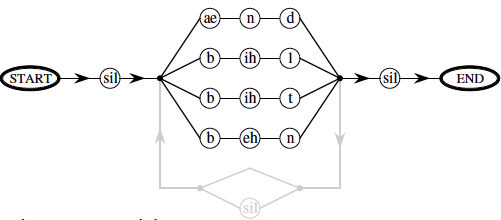
\includegraphics[clip=true, width=0.7\textwidth]{figure/ug.png}
    \bicaption[fig:exp-ug]{}{有限状态语法网络网络以及 unigram和monophone}{Fig}{Finite State Grammar Newwork with unigram and monophone}
\end{figure}

而如果扩展到Bigram和monophone情况下,其语法网络如图~\ref{fig:exp-bg}所示。在每帧上的近似的复杂度则包括内部传递: $W_{\tt ug}\times (P+1)\times N$ 和 外部传递: $W_{\tt ug}\times P + W_{\tt ug}^2$。而如果使用回退back-off语言模型, 词传递大致是 $W_{\tt bg}+W_{\tt bo}\times W_{\tt ug}$。

\begin{figure}[!htp]
  \centering
    \captionstyle{\centering}
    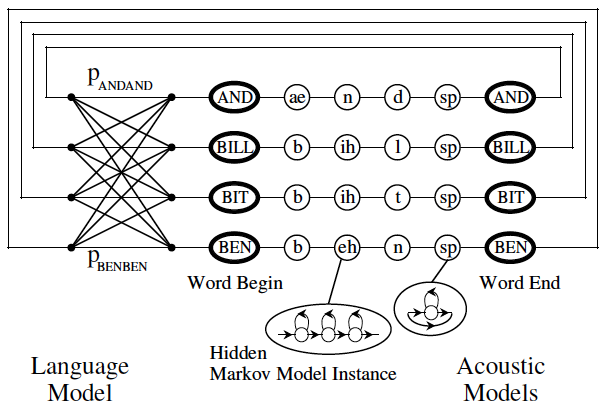
\includegraphics[clip=true, width=0.7\textwidth]{figure/bg.png}
    \bicaption[fig:exp-bg]{}{Bigram和monophone的语法网络}{Fig}{Finite State Grammar Newwork with Bigram and monophone}
\end{figure}


再扩展到Bigram和cross-word triphone 情况下,其语法网络如图~\ref{fig:exp-xwrdbg}所示。在每帧上的近似的复杂度则包括内部传递: $W_{\tt ug}\times (P-2+ P_{\tt prefix}+ P_{\tt suffix})\times N$ 和 外部传递: $W_{\tt ug}^2 + W_{\tt ug}\times (P-2+ P_{\tt prefix}+ P_{\tt suffix})$。

\begin{figure}[!htp]
  \centering
    \captionstyle{\centering}
    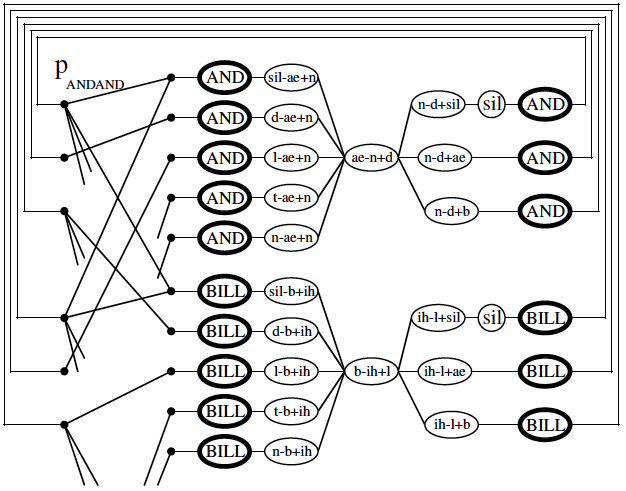
\includegraphics[clip=true, width=0.7\textwidth]{figure/xwrdbg.png}
    \bicaption[fig:exp-xwrdbg]{}{Bigram和cross-word triphone的语法网络}{Fig}{Finite State Grammar Newwork with Bigram and cross-word triphone}
\end{figure}

如果使用Trigram和within-word triphone,其语法网络如图~\ref{fig:exp-tg}所示。在每帧上的近似的复杂度则包括内部传递: $W_{\tt ug}^2\times (P+1)\times N$ 和 外部传递: $W_{\tt ug}^3 + W_{\tt ug}^2\times (P+1)$。
如果是回退back-off LM, 词传递大致是$W_{\tt tg}+W_{\tt bo}^{\tt bg}(W_{\tt bg}+W_{\tt bo}W_{\tt ug}) $。

目前业界最主流的系统使用trigram语言模型和跨词三音子triphone声学模型,该情况下,解码复杂度会变得甚至更大。

总的来说,解码器的搜索空间复杂度与每个词的平均音素数量 P,每个HMM模型的状态个数 N,词表大小$W_{\tt ug}$,ngram历史个数为$W_{\tt ng}$,其复杂度$\mathbb{C}$大致为

\begin{equation}
\label{equ:dec-cmp-space}
 \begin{split}
\mathbb{C}_{space} = O(P\cdot N \cdot W_{\tt ug}^2)+O(W_{\tt ng})
 \end{split}
\end{equation}

另一方面,在传统解码算法中使用第~\ref{chap:intro2-viterbi}章介绍的维特比搜索,其需要在每一帧进行一次完整的搜索空间搜索过程,并由于是动态规划算法,只需要保留上一帧搜索空间内各点的最优结果。因此如果定义搜索空间内每个状态的平均入度为$I$,结果前文分析和公式(\ref{equ:viterbi-cmp}),则最终的复杂度如下,

\begin{equation}
\label{equ:dec-cmp-dec}
 \begin{split}
\mathbb{C} = O(T)\cdot \mathbb{C}_{frame} = O(T)\cdot (O(I) \cdot \mathbb{C}_{space})
 \end{split}
\end{equation}

商用系统中 $W_{\tt ug}$ 和 $W_{\tt ng}$的数量都极其庞大,而T往往可以达到数千帧,因此在下一章节中我们将介绍如何在复杂度如此之高的搜索网络上进行解码搜索。

\begin{figure}[!htp]
  \centering
    \captionstyle{\centering}
    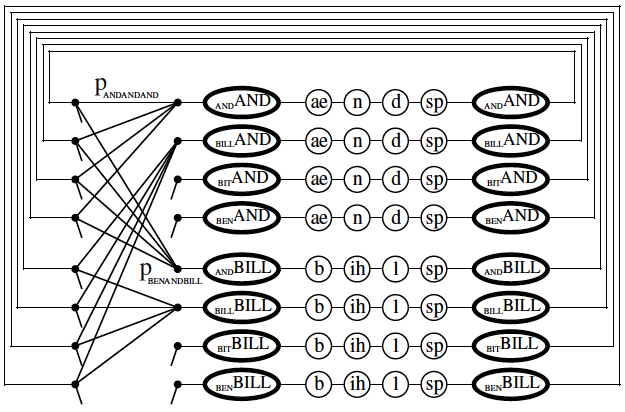
\includegraphics[clip=true, width=0.7\textwidth]{figure/tg.png}
    \bicaption[fig:exp-tg]{}{Trigram和within-word triphone的语法网络}{Fig}{Finite State Grammar Newwork with Trigram and within-word triphone}
\end{figure}

\section{解码器技术综述}
\label{chap:intro2-dec-sum}

\subsection{解码器的技术流派}
\label{chap:intro-lvcsr-decmethod}

\subsubsection{静态和动态的搜索空间构建方法}
\label{chap:intro-lvcsr-decmethod-graph}

根据前面章节讨论,完整的语音信号识别系统由自下而上的五层映射关系组成:语音信号$\mathbf{O}$到HMM状态的观察$\mathbf{s}$,HMM状态到依赖于上下文的音素$\mathbf{c}$,依赖于上下文的音素到单一音素$\mathbf{l}$,音素到单词$\mathbf{w}$,单词到句子。
具体来说公式~\ref{eq:decode}可以进一步展开如下:
\begin{equation}
 \begin{split}
\label{eq:decode-sp}
\mathbf{w}^* = \arg \max_{\mathbf{w} \in \mathcal{H}} \max_{\mathbf{s}} P(\mathbf{s}|\mathbf{w})p(\mathbf{O}|\mathbf{s})P(\mathbf{w}) \\
= \arg \max_{\mathbf{w}} \sum_{\mathbf{l}} \sum_{\mathbf{c}} \sum_{\mathbf{s}}
p(\mathbf{O}|\mathbf{s}) \cdot
P(\mathbf{s}|\mathbf{c})\cdot P(\mathbf{c}|\mathbf{l})\cdot P(\mathbf{l}|\mathbf{w}) \cdot 
P(\mathbf{w})
 \end{split}
\end{equation}
其中展开后式子每一项分别对应上述的五层映射关系。
在识别之前不能知道语音信号的观察,因此需要在解码过程中动态地建立观察到的语音信号的HMM状态的映射,并且还需要实时计算相应的声学分数。对于从HMM状态到依赖于上下文的音素,依赖于上下文的音素到音素,音素到单词的三级映射关系,一旦确定了发音字典$\mathcal{H}$,语言模型$P(\mathbf{w})$,和声学模型,它们就不会改变。为了追求解码效率,人们通常将它们静态编译成解码网络。对于没有任何约束的大词汇量连续语音信号的识别任务,可以以任何方式将单词组织成句子,因此原则上,单词 - 句子映射关系只能在解码过程中动态建立。然而,由于表征单词和单词之间的关联度(概率)的N-gram语法模型在解码之前已经存在并且是有限集,因此在实践中,语言模型得分计算可以以不同方式实现。在语音信号识别领域,根据解码器中语言模型的表示,语言模型状态获取和语言模型得分计算方法,解码器通常分为两大流派:
\begin{itemize}
\item 动态网络解码器: 在动态网络解码器中,解码网络仅包含发音字典和声学
模型,不会含有语言模型任何信息。 语言模型状态在解码过程中还要随着词与词相连
成句而动态地生成、语言模型分数通过去查表的方式动态地获取。这类解码器的典型
代表是基于发音前缀树(Pronunciation Prefix Tree, PPT)~\cite{woodland1994large}网络解码器。
\item 静态网络解码器: 在静态网络解码器中,解码网络不仅包含发音字典和声
学模型,也包含完整的语言模型分数。 语言模型状态以及状态转移以WFST的形
式合成到解码网络中去, 语言模型分数则作为状态转移概率存储于边上。解码时,
仅需逐边积累整条路径状态转移概率便可获得语言模型分数。这类解码器的典
型代表是基于加权有限状态转换器(WFST)~\cite{mohri2002weighted}的解码器。
\end{itemize}

作为一种时空变换策略,静态网络解码器通常可以通过仔细优化实现更快的识别速度,但缺点是构建的解码网络太大,特别是在高阶语言中。随着硬件设备的发展,存储器对解码网络大小的限制逐渐减少,本论文工作主要基于静态网络解码器,将在第\ref{chap:intro2-wfst}章节对其理论做进一步介绍。

\subsubsection{同步和异步的搜索算法}
\label{chap:intro-lvcsr-decmethod-search}

除了根据解码网络的结构进行分类之外,还可以根据搜索最优路径的不同方式将解码器划分为时间异步搜索解码器和时间同步搜索解码器:

\begin{itemize}
\item 时间异步搜索解码器: 在较老的解码器,例如: IBM ViaVoice 中, 采用深度优先方式在解码网络中搜索最优词序列, 是一种时间异步搜索。由于这类解码
器在解码过程中需要用到一些后进先出的缓冲区(即:堆栈)来保存扩展得到词识别假设,所以也常常被称为堆栈解码器(Stack decoder)~\cite{paul1992efficient}。 
与时间同步搜索相比,优点在于通过选择适当的启发函数,搜索可以控制于最佳路径附近,并且提高了搜索效率。但这也造成了它的主要缺陷:1)启发函数综合声学和语言分数,有时需要“未来”路径信息,因此很难获得; 2)因为它是时间异步搜索,所以搜索过程产生的路径长度各不相同,使得修剪很难实现。因此,当前的堆栈解码很少用于直接解码语音信号的观察,而更多地用作用于从字图生成N-Best结果的后处理中。
\item 时间同步搜索解码器:时间同步搜索是目前解码器设计和实现的主流方法,也称为帧同步搜索。它使用广度优先方法找到与来自解码网络的输入特征序列最佳匹配的状态序列,以便获得相应的最佳音素序列和字序列。这种类型的解码器通常使用维特比算法或令牌传递算法~\cite{woodland1994large}实现。 
\end{itemize}

时间异步的搜索算法还包括多遍解码算法。多遍解码算法通常在每次解码过程中对之前的搜索空间进行剪枝,缩小空间大小,而后将压缩后的搜索空间交给下一次解码算法,进行进一步搜索,直到最终得到最佳结果。
为在搜索中利用各种各样的知识源,通常要进行多遍搜索,第一遍要使用代价较低的知识源,产生一个候选序列列表或词候选网格,在此基础上再进一步进行使用代价高的知识源的第二遍搜索来得到最佳路径。这里的知识源包括声学模型、语言模型和音标词典,这些可以用于第一遍搜索。为实现更准确的语音识别,往往要利用一些代价更高的知识源,如高阶的上下文相关的N-Gram语音模型、词间混淆相关模型、分段模型或语法分析算法,进行重新打分。目前主流的实时大词汇连续语音识别系统许多都使用这种多遍搜索策略。
与单遍搜索(1-pass)相比,多遍搜索具有优点和缺点,并且它也在实践中使用。多遍搜索的支持者认为:第一遍粗搜索可以大大减少解码空间,使得在后续解码过程中使用更精细的语言模型和声学模型成为可能,避免了单遍解码器中的时间和空间限制。 。单遍搜索的支持者认为在多遍解码中存在三个主要问题:1)由于第二遍解码必须等待第一遍解码,因此多遍搜索难以应用于实时解码。 2)每次通过解码引入了不可恢复的修剪误差,其不能被后续解码中使用的任何模型补偿。要解决这个问题,我们仍然需要努力研究单遍搜索算法。最好直接进行单遍解码器。 3)多次解码器的每次解码中使用的特征,声学模型,语言模型和搜索算法是不同的。

解码器不仅算法复杂,而且需要高工程能力和技能。在开发完成后,通常需要大量的人力和时间进行调整。因此,各种研究机构和商业公司都有自己的解码器实现细节。它就像它一样深。尽管如此,世界上仍有一些用于学术研究的开源解码器可以作为研究的基础。该表列出了比较知名的那些。这些解码器的网络结构和解码算法不同,但由于学术研究的目的,大多数速度优化都比较差。


\begin{table}[thbp!]
  \caption{\label{tab:perf-compare} {\it  知名开源解码器 } }
  \centerline{
    \begin{tabular}{c c  c c}
      \toprule
      解码器 &  研发机构 & 网络结构 & 搜索算法 \\
      \midrule
      HDecode & 英国剑桥大学 & 动态,发音前缀树 & 单遍, 令牌传递 \\
        Sphinx &美国卡内基梅隆大学 &动态,发音前缀树 &单遍, 令牌传递 \\
        RASR &德国亚琛工业大学& 动态, 发音前缀树 &单遍, Viterbi \\
        Juilus & 日本京都大学 & 动态, 发音前缀树 & 两遍, 前后向搜索。\\
        Juicer & 瑞士IDIAP & 静态, WFST & 单遍,令牌传递 \\
        Kaldi & 美国约翰霍普金斯大学 & 静态, WFST & 两遍,令牌传递     \\
\bottomrule
    \end{tabular}
  }
\end{table}


\subsection{主要模块和核心算法}
\label{chap:intro-lvcsr-decmodule}

\subsubsection{解码器框架}

图~\ref{fig:dec_arch}给出了典型解码器结构。不论是哪种类型解码器通常都包含网络生
成、分数计算、搜索、剪技与路径管理等部分,它们的功能逐一介绍如下。

\begin{figure}[!htp]
  \centering
    \captionstyle{\centering}
    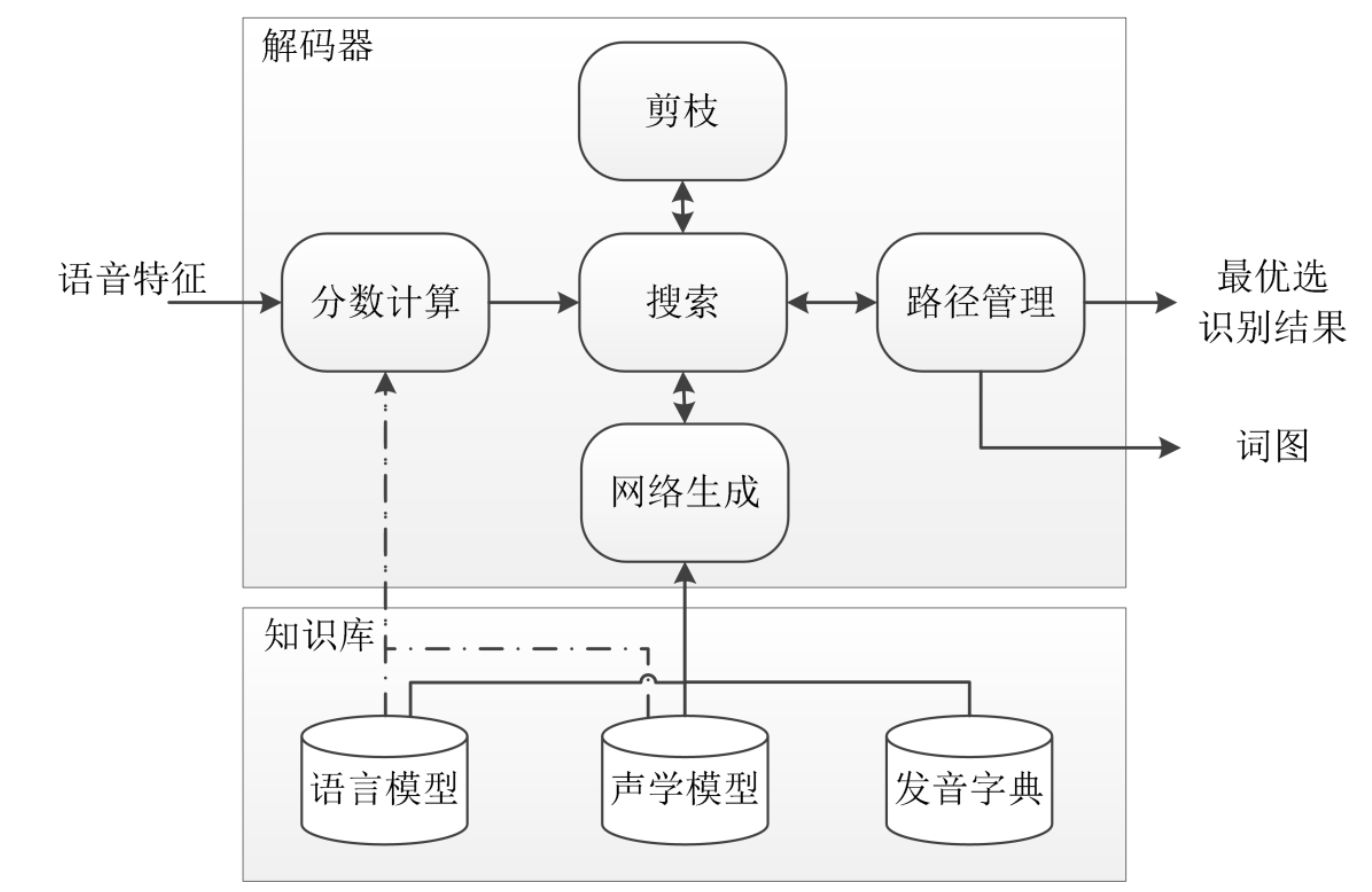
\includegraphics[clip=true, width=.9\textwidth]{figure/dec_arch.png}
    \bicaption[fig:dec_arch]{}{通用解码器架构}{Fig}{General Architecture of ASR Decoder}
\end{figure}


\subsubsection{基于加权有限状态机的网络生成算法}
\label{chap:intro2-wfst}

网络生成模块主要负责构建解码搜索空间。搜索空间(也称为解码网络)通常与音素HMM或HMM状态连接,从语言模型,发音词典,声学模型和其他相关知识源编译。大词汇量连续语音信号解码网络的识别系统由各种知识源组成,形成搜索空间,一般可分为动态构造的解码网络和静态网络。基于动态网络解码器,前缀树发音字典用作搜索网络。语言模型通过动态查询将得分引入解码过程,然后通过重新输入字典树或字典树副本来搜索整个解码网络~\cite{young2002htk}。
动态网络解码器主要优势在于,由于字典和语言模型是分离,其占用内存极少,这个特点在以往移动网络技术和硬件技术不发达的时代,尤其是在嵌入式设备上内置解码器的时代,占有着绝对优势。但是动态网络的缺点是它解码速度较慢,时间复杂度较高,这也使其愈加难以满足当前海量语音信号的识别请求。
随着移动互联网和嵌入式设备的普及以及云技术的发展,语音信号的识别应用已发展为仅在嵌入式设备上保持简单的前端,而识别系统仍保留在服务器云中。此时,反映了基于WFST的静态网络解码器的快速优势。较短的识别时间允许服务器每单位时间接受更多的识别任务,因此静态编译的解码网络更适合于大量语音信号识别任务。

在LVCSR任务中,解码网络通常非常大。因此,网络结构需要采用各种手段来优化网络结构,并在不改变网络功能的情况下尽可能地减少网络中的节点和边数量。解码网络是解码器的基础,并确定在解码器的其他部分中应该使用哪种方法。在静态网络解码器中,解码网络不仅包含发音字典和声学模型,还包含完整的语言模型。语言模型状态和状态转换以有限状态机的形式合成到解码网络中,并且语言模型得分被存储为边上的状态转移概率。当解码时,仅通过累积整个路径状态转移概率可以获得语言模型得分。这类解码器的典型代表是基于加权有限状态转换器(WFST~\cite{mohri2002weighted}的解码器。

WFST最开始由AT\&T实验室Mohri和Riley等人在1997年引
入语音信号的识别领域。并且在理论上发展了确定化、最小化等一系列网络优化算法,为语音信号的识别的应用打好了理论基础。
具体来说,上文讨论的解码搜索问题基于公式(\ref{eq:decode-sp}),其中$p(\mathbf{O}|\mathbf{s})$由声学模型建模得到,
语音识别的其他各模型组件分别用如下方式进行WFST构建:

\begin{itemize}
\item N-gram语言模型在WFST中表示为G,在公式(\ref{eq:decode-sp})中表示为$P(\mathbf{w})$。根据N-gram语言模型的含义,它提供了单词历史的当前单词概率。语言模型需要具有记录最多N个单词的历史的信息。但是,当识别语音信号时(即,输入和输出是其符号集的单个元素),WFST应用程序不允许使用字符串输入和输出。因此,不可能在G构造过程的输入和输出上表达其历史,而是记录该状态的历史。另一个问题是N-gram模型的回退(Back-off),当语言模型训练语料未出现某一个N元词组的时候,就会以一个回退的(N-1)元模型概率乘以一个系数来替换。这部分表示为一个带有着权重但是输入为空的状态跳转边。

\item 字典在WFST中被表示为L,在公式(\ref{eq:decode-sp})中表示为$P(\mathbf{l}|\mathbf{w})$。
字典实际上是发音规则的表示。最简单的方法是列出开始状态和结束状态之间每个单词的发音。同时,由于在与语言模型合成时连接了单词和单词,因此无法达到终止状态,并且需要将闭合边从终止状态连接到开始状态以形成闭环。针对字典的同发音问题,Mohri在文献~\cite{mohri2002weighted}中提出对于不同词的同发音发音
序列加入一组辅助符号,这样对于同发词语,其环路的输入符号序列就不再相同,可以确保字典的可确定化。

\item 上下文相关声学模在WFST中被表示为C,在公式(\ref{eq:decode-sp})中表示为$P(\mathbf{c}|\mathbf{l})$。
一个上下文相关triphone模型一般表示为a-b+c,其中b是中心音素,
a和c为其前后上下文音素~\cite{seide2011conversational}。用WFST表示triphone模型实际上是在把三音素和单个音素之间进行对应,其输出就和发音字典的输入做相互对应,由此可以进行进一步合成。

\item 隐马尔可夫模型在WFST中被表示为H,在公式(\ref{eq:decode-sp})中表示为$P(\mathbf{s}|\mathbf{c})$。
HMM模型天然具有多个的状态跳转特性,所以可以直接将其构建为多个WFST状态。隐马尔科夫模型的转移概率于是被转化为WFST的权重。而WFST输入是隐马尔科夫模型的状态索引,输出是该隐马尔科夫模型所表示的triphone建模单元。
\end{itemize}

当各个知识源WFST组件被构建完毕以后,可以利用WFST合成算法和优化算法将各组件最后进行合并和最终优化。如下:
\begin{equation}
HCLG = min(det(H \circ min(det(C \circ min(det(L \circ G))))))
\end{equation}

最终生成的WFST包含了所有的知识源,它是一个输入为HMM状态$\mathbf{s}$,输出为词语$\mathbf{w}$的WFST网络,用于建模$p(\mathbf{s}|\mathbf{w})\cdot p(\mathbf{w})$。结合声学模型建模的$p(\mathbf{O}|\mathbf{s})$概率,后文所讨论维特比搜索就在该WFST网络上面进行。

\subsubsection{分数计算}
\label{chap:intro2-score}

分数计算模块计算输入特征序列声学和语言分数,并将它们提供给搜索模块以供使用。应该计算哪个分数与解码网络结构和搜索算法有关。例如,在静态网络解码器中,语言模型得分已经被编译到解码网络中,因此只需要计算声学得分;对于动态网络解码器,除声学分数外,还需要计算语言模型分数。分数计算的研究主要集中在如何实现分数的快速计算。对于声学分数,通常执行以下三个方面:

\begin{itemize}
\item 硬件加速。
%
利用 CPU 矢量计算器~\cite{kanthak2000using}
或者图形处理器(Graphics Processing Unit, GPU)~\cite{chong2009fully}
加速分数计算。这类方法通常来说不会带来计算误差(与硬件实现相关),所以对识别准确度没有影响。
\item 模型简化。
为了减少声学模型推理的计算开销,研究人员们提出了一系列效率更高的声学模型,包括一些比较新颖的神经网络结构~\cite{xue2014singular,peddinti2018low}, 跳帧~\cite{pundak2016lower,zhc00-chen-is16,zhc00-chen-tasl2017}
和端到端系统~\cite{audhkhasi2017direct,e2e-2018}。
%frame sub-sample or PSD, novel model, SVD, quantization, ...
这还包括采用复杂度更小、参数更少的分类器模型,或通过聚类和参数共享减
小模型复杂度。例如采用半连续 HMM~\cite{huang1990semi} 替代连续 HMM,以及传统的参数共享方式~\cite{young2002htk}亦属此类。这类算法一般都会带来识别准确度上面的损失,所以需要在
识别准确度、模型复杂度和计算速度之间做好一定的权衡。
\item 算法优化。 对声学分数的计算过程进行简化。这类方法一般是对声学分数进行近似计算,所以必然会带来一定识别准确度损失。一般而言, 衡量一个近似算法是否可用的标准是看其带来相对识别准确度损失是否可控制在5\%以内~\cite{cai2009efficient}。
\end{itemize}

对于语言分数计算,当采用 N 元文法模型时,通常从两个方面进行加速: 1)
减小每次查表操作上面的耗时,典型方法是采用最小完美哈希(Minimal Perfect Hash,
MPH)表实现语言模型的存储与查取~\cite{li2007fast,cardenal2002fast}; 2) 引入分数缓存~\cite{huijbregts2008fast}减少查表熵的次数。

\subsubsection{帧同步的维特比解码算法}
\label{chap:lsd-review-fsd}

在大词汇量连续语音识别(large vocabulary conversational speech recognition, LVCSR)中,解码算法的目标是找到最佳的词序列。通过应用字典和语言模型将词序列映射到标签序列,解码公式可推导如下:
\begin{equation}\label{eq:asr-dec}
        \mathbf{w}^*=\mathop{\arg\!\max}\limits_\mathbf{w} \{
        P(\mathbf{w})p(\mathbf{x}|\mathbf{w})
        \}=\mathop{\arg\!\max}\limits_\mathbf{w} \{
        P(\mathbf{w})p(\mathbf{x}|\mathbf{l}_\mathbf{w})
        \} %\nonumber
     \end{equation}
其中,$\mathbf{w}$是词序列,${\mathbf{w}}^*$ 是最佳词序列。$\mathbf{l}_{\mathbf{w}}$ 表示 $\mathbf{w}$通过映射得到的标签序列,如NN-HMM系统中的上下文相关音素。

以CTC为例:
\begin{equation}\label{eq:ctc-with-prior}
        \mathbf{w}^*=\mathop{\arg\!\max}\limits_\mathbf{w} \left\{
        \frac{P(\mathbf{l}_\mathbf{w}|\mathbf{x})P(\mathbf{w})}{P(\mathbf{l}_\mathbf{w})}
        \right\}
     \end{equation}
     \begin{equation} \label{eq:ctc-dec}
    = \mathop{\arg\!\max}\limits_\mathbf{w} \left\{
        P(\mathbf{w})
        \mathop{\max}\limits_{\mathbf{l}_\mathbf{w}} \frac{P( \mathbf{l}_\mathbf{w}|\mathbf{x} )}{P(\mathbf{l}_\mathbf{w})}\right\}
     \end{equation}

这里以单音素的CTC为例(CTC标签符号集合包括音素标签和$\tt blank$符号)。   $P(\mathbf{l}_\mathbf{w})$是音素序列的先验概率。
对于某个特定的CTC标签序列,其前向概率可定义\cite{graves2006connectionist}并近似为:

        \begin{equation} \label{eq:fwd-ctc}
        P(\mathbf{l}|\mathbf{x}) =
        \sum_{\pi\in\mathcal{B}(\mathbf{l})} %\pi:\pi \in L',\mathcal{B}(\pi_{1\mathord{:}T})=\mathbf{l}
           {\prod_{t=1}^{T}{y^{t}_{\pi_{t}}}}
        \cong \mathop{\max}\limits_{\pi\in\mathcal{B}(\mathbf{l})}
           {\prod_{t=1}^{T}{y^{t}_{\pi_{t}}}}
        \end{equation}


其中, $\mathcal{B}$的定义见公式\ref{equ:ctc-b}。
因此,公式\ref{eq:ctc-dec}可进一步被推导为如下的帧同步维特比束搜索(frame synchronous Viterbi beam search, FSD)。这里,整体优化搜索空间-WFST,在每一帧都需要被遍历。

              
    \begin{equation} \label{eq:viterbi-app}
    %\begin{split}
       \mathbf{w}^* \cong\mathop{\arg\!\max}\limits_\mathbf{w}
       \left\{\!
       P(\mathbf{w})
       \mathop{\max}\limits
       _{\!\!\pi\in\mathcal{B}(\mathbf{l})}
       \frac{1}{P(\mathbf{l}_\mathbf{w})}
       \prod_{t=1}^{T}{y^{t}_{\pi_{t}}}
      \right \}
    \end{equation}

  
在FSD框架中,将特征帧的数量除以语句的长度定义为特征速率,标签输出数量除以语句的长度定义为标注速率,而WFST解码的帧数除以语句的长度定义为解码速率。该框架中,三个速率均相等。也就是说, $\prod_{t=1}^{T} y^{t}_{\pi_{t}}$  与帧t有关,而最大迭代次数则与序列可能的对齐方式和词汇量的大小有关。 因此,解码复杂度$\mathbb{C}_{FSD}$ 可表示为:
  \begin{equation}
\label{equ:complex-fsd}
\begin{split}
\mathbb{C}_{FSD} =  O(T) \cdot \mathbb{C}_{frame}
\end{split}
\end{equation}
其中T是语句中帧的数量,I和$\mathbb{C}_{frame}$定义参见公式\ref{equ:dec-cmp-dec}。

\subsubsection{令牌传递算法}

解码搜索模块负责在解码网络上搜索得到最优路径。不论是静态网络解码器还是动态网络解码器,目前都以令牌传递算法~\cite{young1989token}为主流的搜索算法。

令牌传递是上文讨论的帧同步的维特比算法的另一个更通用和简单的实现。在算法中,每个HMM状态可以与令牌(Token)相关联,令牌存储令牌所经历的历史路径和路径得分直到当前帧。解码是根据状态转换(即,沿着解码网络的边)将令牌从解码网络的初始状态传递到终止状态的过程。每个帧令牌向前传递一次,同时传递令牌得分和路径信息,并在多个令牌同时传递到状态时进行令牌合并,仅保留具有最高得分的令牌。在处理完所有帧之后,获得最佳路径和最佳路径得分。简化的算法流程如算法\ref{code:tokpass}所示。


\begin{algorithm}[ht]
\caption{令牌传递算法\ {(Inputs:  \textcolor[rgb]{0,0.5,0}{初始Token; 声学分数矩阵;总帧数})}}
\label{code:tokpass}
\begin{algorithmic}[1]
\Procedure{Token Passing} {startTok, amScores, T}
\State    $\bullet$ \textrm{算法初始化}
\State Queue = [startTok]
\State stateMap=$\{\}$;
\State    $\bullet$ \textrm{令牌传递}
\For {t in T} \Comment \textcolor[rgb]{0,0.5,0}{每一帧}
\For{curTok in Queue} \Comment \textcolor[rgb]{0,0.5,0}{每一个上一帧的Token}
\For{arc in curTok.arcs}  \Comment \textcolor[rgb]{0,0.5,0}{每个Token的出边}
\State amScore=amScores[t][arc.inId];
\State nextScore=curTok.score+amScore-arc.weight;
\State nextState=arc.nextState;
\State    $\bullet$ \textrm{令牌合并处理}
\If {nextState $\not\in$ stateMap}  \Comment \textcolor[rgb]{0,0.5,0}{如果该WFST State无Token}
\State newTok=Token(nextScore, curTok);
\State stateMap[nextState]=newTok;
\EndIf
\If {stateMap[nextState].score $<$ nextScore}   \Comment \textcolor[rgb]{0,0.5,0}{存在但分数小}
\State stateMap[nextState].score=nextScore;
\State stateMap[nextState].prevTok=curTok;
\EndIf
\EndFor
\EndFor
\State $\bullet$ \textrm{下一帧的预处理}
\State Queue=stateMap.toList();
\State stateMap.clear();
\EndFor
\EndProcedure
\end{algorithmic}
\end{algorithm}

令牌传递算法的优点是可以方便地在令牌上保存其他信息以便在状态节点之间进行传递,从而实现更复杂解码过程,例如: 为了生成词图,在令牌合并后, 不是将次优令牌直接丢弃,而是作为其他候选路径保存于合并后的令牌之上。

\subsubsection{剪枝}

观察公式(\ref{equ:dec-cmp-dec}),在LVCSR中,搜索空间太大而无法对整个解码网络执行完全搜索。剪枝用于消除解码过程中的低分数路径,从而减少计算量并确保不降低识别性能。根据解码器设计,剪枝可以应用于搜索的各个阶段(例如,开始或结束),或者可以应用于各种级别(例如,单词级别,音素级别,状态级别,令牌级别),但是可以归纳为三个基本类别:

\begin{itemize}
\item 束剪枝(Beam pruning) :束剪枝保留与最优路径分数较近的次优路径。
令 $v(t,j)$ 表示第 t 帧位于状态 j 最优路径分数,则第t 帧的最优路径分数为:
\begin{equation}
v_{max}(t)=max_s v(t,s)
\end{equation}

令 $f$ 为剪枝阈值(又称为束宽),则束剪枝只保留所有满足下式的路径:
$v(t,j)>v_{max}(t)\cdot f$
\item 直方图剪枝(Histogram pruning) :与束剪枝不同,直方图剪枝仅保留分
数最高 K 条路径, K 为设定剪枝阈值。之所以称为直方图剪枝是因为该方法
可以采用直方图统计高效地实现~\cite{pylkkonen2005new}。

\item 向前预测声学和语言分数~\cite{soltau2009dynamic,nolden2012search}:
通过算法的改进,合理地预测未来的声学和语言分数,并据此提前对可能性进行剪枝,也是一种主要的优化方式。
\end{itemize}

以直方图剪枝为例,由于每帧只需要考虑K条路径,并且上一帧只保留K条路径,因此如果定义搜索空间内每个状态的平均出度也为$I$,复杂度公式(\ref{equ:dec-cmp-dec})中的$\mathbb{C}_{frame}$将显著减少如下,

\begin{equation}
\label{equ:dec-cmp-space2}
 \begin{split}
\mathbb{C}_{frame} = O(K \cdot I )
 \end{split}
\end{equation}


\subsubsection{路径管理和词图}

路径管理模型主要作用是用于对搜索过程中得到的路径链表进行回溯,获取最优路径、
N-Best 结果和词图。同时,它也负责对剪枝过程中所剪掉的较差路径进行内存回收等操作。

\begin{figure}[!htp]
  \centering
    \captionstyle{\centering}
    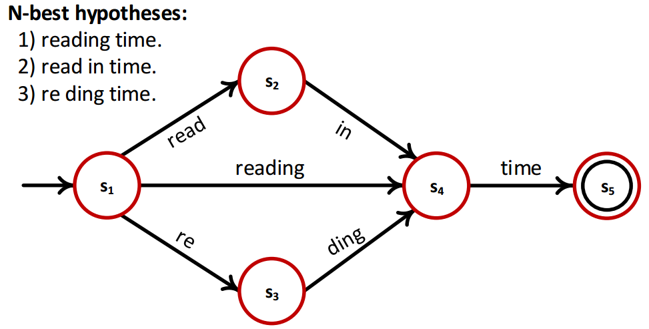
\includegraphics[clip=true, width=0.6\textwidth]{figure/lattice.png}
    \bicaption[fig:lattice]{}{N-Best候选序列和词图}{Fig}{N-Best Hypothesis and Lattices}
\end{figure}


由于N-Best候选序列中往往存在大量的公共部分(比如图~\ref{fig:lattice}中的“time”这个词),因此将公共部分优化在一起进行表示,也就是将多个候选序列转变成一张图来进行存储,将会更加紧致。在语音信号的识别中,这样一张图就称为词图。词图的生成所带来的额外消耗与生成N-Best候选序列类似。具体来说,其往往要求在解码过程中做令牌合并时,保留多个历史令牌记录。在记录完词图后,还需要词图剪枝步骤,其将冗余和无法连通边及其相应结点删去,得到最终比较紧致的词图。

词图具有较多用途,比如:词图语言模型重打分,鉴别性训练,置信度计算,混淆网络生成等。
因此相较于N-Best候选序列,词图的处理往往是语音信号的识别系统中的一个标准模块。


\subsubsection{语音识别中的置信度}
\label{sec:intro-cm}

% TODO: ref http://hci.stanford.edu/research/speech/
在最近十年时间,自动语音识别 (ASR) 取得了非常显著的成功。但是当语音识别系统由实验室产品转向真正的应用时,即使是最好的语音识别系统,仍然会不可避免地产生一些识别中的错误 \cite{ruan2016speech},也就是说ASR系统的输出总会包含或多或少的一些各种各样的错误。
因此,在真实的应用场景中,人们一般需要ASR系统能够自动评估自身的可靠性和发生错误的概率,而这些都由系统自身得出。

在语音识别中,置信度(CM)就是提出来进行这种类型的可靠度评估的\cite{jiang2005confidence}。这类模型可以被分为如下几种类别:

\begin{itemize}
    \item {\em 基于用于建模的特征的置信度}.
    基于ASR识别过程的特征被称为用于建模的特征,而它的概率分布在识别正确和识别错误时会产生显著的不同。
    CM可以由它们之中的一个或两个来组成,比如对归一化后的声学分数 \cite{hu2013new}, 时长 \cite{ma2011fusing}, 局部交叉熵 \cite{falavigna2002acoustic}。
    但是,这些用于建模的特征并不完美地表示解码的过程 \cite{jiang2005confidence}. 所以一些分类器模型也可以考虑被加入到这些用于建模的特征上,比如 CRF \cite{seigel2013confidence}, 深度学习 \cite{yu2011calibration}, 等等。但是这些模型仍然不够完美。首先各个用于建模的特征之间并不完全独立,其次它需要额外的训练阶段,并假设训练数据与测试数据匹配。
    %feature and model method weakness:
    %need further training stage; hard to formulate; depend on scenario of training data, assuming scenario of test and training data is the same

    \item {\em 基于后验概率的置信度}.
    另一种方法将ASR过程建模为 {\em 最大后验概率} (MAP) 的决策过程。给定整个句子后的ASR输出的后验概率可以用来表示CM。许多方法研究了如何对归一化项进行建模,比如 filler 模型 \cite{young1994detecting}, 词图\cite{wessel2001confidence} 和混淆网络(CN) \cite{evermann2000large}。然而,ASR解码器通常设计用于寻找最优的首选路径,这使得它所得到的词图并不完美,同时会导致CM的建模并未较好地归一化 \cite{yu2006maximum}.
    %filler/lattice/cn

\end{itemize}


\section{解码器研究中的待解决问题}
\label{chap:intro2-dec-future}
\subsection{研究现状总结}
\label{chap:intro2-dec-sumcur}

语音识别技术虽然相比多年以前已经有了长足的进步,但是在实际应用中还有很多困难需要处理。其中一个最主要难题就是语音识别推理搜索问题。
%
% 做什么事情
语音识别既是模式识别问题又是相应的推理搜索问题。前一个问题在数学上表示和描述了各种语音和语言现象,并且基于统计学习模式识别框架执行建模,该框架确定了语音识别系统可以实现的识别准确度的上限。在给定模型的情况下,后一问题研究如何使输入语音与模型匹配并推断最佳识别结果,其确定识别速度和实际可达到的识别准确度。在语音识别的推理搜索阶段,解码器功能组合声学模型以计算声学特征概率和语言模型计算的语言概率以获得最大概率词序列。
在语音识别推理搜索阶段,解码器是语音识别系统的核心和灵魂,所有信息都收集在这里。它将来自不同来源,不同层次和不同性质的知识和信息联系起来,以便它们相互补充并获得正确的语音识别结果。因此,如何有机地整合各种不同的信息是解码网络和解码算法设计中必须仔细研究和解决的问题。
从解码器功能的角度来说,它不仅是语音识别研究中各种理论,模型和算法的验证。
正确性和准确性的基本实验平台也是构建实际系统的基础所在。因此,在解码器的设计中必须平衡研究的便利性和工程的实际应用。


% 近来深度学习下发展现状和缺陷
近年来,深度学习模型被引入到语音识别声学和语言建模中以取代传统的分类器,显着提高了模式识别问题的准确性。在基于深度学习语音识别中,语音识别的推理搜索问题并没有得到根本改变。因为在该框架中,只有分类器得到了改进。
基于加权有限状态机(WFST)的推理搜索问题静态搜索空间构造技术~\cite{mohri2002weighted}和帧同步维特比(Viterbi)网络搜索算法~\cite{forney1973viterbi}仍是目前性能最好解决方案。该类系统存在的一系列显著缺陷包括:
\begin{enumerate}
\item 目前,语音识别系统基于多知识源建模结果,并对输入音频进行推理搜索。建模和推理搜索过程非常复杂,知识来源的划分依赖于强大的先验知识。大规模或非标记语音数据收集以及基于并行的深度学习技术使得构建直接模拟语音数据和文本序列的端到端模型及其相应的识别和推理搜索算法成为可能。当前的解码框架没有这种设计。
\item 
该种方案基于传统的混合高斯-隐马尔科夫模型(GMM-HMM)的声学模型和N元文法(N-gram)的语言模型而提出,针对目前性能最好的基于深度学习的声学模型和语言模型的研究并不充足,如何将新型的声学和语言模型引入该框架;如何充分发挥模型性能的同时改善推理速度;如何基于多知识源给出可靠的推理置信度算法,都是有待解决的问题。
\item 
该种方案基于对语音识别中各知识源(声学、语言、语义等)进行搜索空间的预先构建及整体优化,导致最终得到的搜索空间巨大,包括离线构建、在线使用、动态修改等各环节算法的计算量和内存消耗都非常大,是阻碍语音识别应用场景扩展的一个重要原因。旨在解决该问题,针对新型声学和语音模型的搜索空间整体优化研究尚不充分,而基于推理中间状态对搜索空间进行动态优化的研究几乎处于空白。
\end{enumerate}
因此,尽管基于深度学习模型,加权有限状态机和基于帧的维特比网络搜索算法的深度学习已经发展到基本可用水平,但是精度仍然不能满足人类之间的正常交流要求。速度限制也使得语音识别无法在低成本和低功耗的解决方案上工作,这些解决方案一起阻碍了语音识别技术的大规模商业应用。

\subsection{发展机遇和亟待解决问题}
\label{chap:intro2-dec-todo}
\begin{enumerate}
\item 基于GPU并行计算提高解码搜索速度。

随着深度学习的发展和计算设备的更新,基于GPU的并行计算是一种潜在的针对语音识别计算的加速方式。针对声学模型推理,由于大部分计算量集中在矩阵形式的运算,因此它易于通过将类似于训练过程中\cite{vesely2010parallel}的序列批处理~\cite{dixon2009harnessing} 引入模型推理阶段,以加速运算速度。
但是,基于GPU并行计算的解码搜索并不容易实现。本质上它不再是一个易于并行的矩阵运算问题,而是一个图上最优路径的搜索问题。尽管一些研究在小型语言模型上取得了一定成功~\cite{you2009parallel},但这些系统仍然受制于两部分缺陷:i) 由于GPU显存有限,这些方法并不能有效利用较大的商用语言模型。
ii) 这些方法并不通用,常常受制于特定的声学或语言模型,并且没有词图生成功能。我们将在第~\ref{chap:gpu}章节对该方向进行研究。

\item 基于端到端建模降低解码搜索复杂度。

近来神经网络的发展使得更强的上下文和历史建模效果成为可能\cite{sak2014long,qian2016very}。同时,更多的标注数据也进一步缓解了模型的稀疏性和泛化问题。这些进展使得研究人员们有可能在更大的模型粒度上-从帧到整个序列层面~\cite{amodei2015deep,soltau2016neural,collobert2016wav2letter,sak2015fast,chan2016end}进行序列分解。在这些研究中,标签速率小于特征速率,但解码速率仍然等于特征速率。针对端到端模型的特性,特征层面的搜索过程可以考虑被修改为标签层面,即搜索空间是由不同历史的标签组成的,使得解码速率等于标注速率,从而小于特征速率。由于标签速率显著小于特征速率,这样做的好处是将带来搜索复杂度的大幅下降,从而得到搜索速度的大幅提升。我们将在第~\ref{chap:lsd}章节对该方向进行研究。

\item 基于端到端建模简化和统一解码推理框架。

由于不同ASR应用之间不同的搜索空间大小和效率要求,当前业界最优的置信度及其相应的解码算法在不同应用上具有不同架构,这些不同应用包括:关键词检测,基于上下文的语音识别和大词汇连续语音识别。要为所有的ASR应用设计一套统一的推理搜索框架,并取得最好的性能和速度,是一项非常有挑战的研究。这里面的关键点在于: i) 如何对最佳识别结果进行规范化,以得到对该最佳结果的置信度估计,也就是置信度中的归一化项的建模   ii) 如何保证在低功耗设备中的计算量控制在一个较小范围内,这对于置信度中的归一化项建模尤其具有挑战。借助上面提到的端到端建模,一方面可以对建模中的归一化项进行统一的较复杂的计算,另一方面可以有效降低上述计算中的复杂度。我们将在第~\ref{chap:lsd-apply}章节对该方向进行研究,将端到端建模所带来的解码搜索优化应用到更多领域中。

\end{enumerate}
\section{本章小结}
\label{chap:intro2-sum}


本章回顾了语音信号识别和推理搜索阶段的搜索和解码部分的基本内容和方法。解码器将由声学模型计算的声学特征概率与由语言模型计算的语言概率组合,以获得最大概率词序列。在语音信号的识别和推理搜索阶段,解码器是语音信号识别系统的核心和灵魂,并且在此收集所有信息。它将来自不同来源,不同层次和不同性质的知识和信息联系起来,使它们相互补充,得到正确语音信号的识别结果。因此,如何有机地整合各种不同的信息是在解码网络和解码算法的设计中必须仔细研究和解决的问题。
从解码器的作用来看,它不仅是验证语音信号识别中各种理论,模型和算法正确性的基本实验平台,也是构建实际系统的基础。因此,在解码器的设计中,还需要考虑研究的便利性和工程的实际应用。

本章中重点总结了目前解码器的研究现状及存在的缺点和实现难点。后续几章我们的改进工作将具体针对所有这些目前存在的问题进行展开。
